%%%%%%%%%%%%%%%%%%%%%%%%%%%%%%%%%%%%%%%%%%%%%%%%%%%%%%%%%%%%%%%%%%%%%%%%%%%
%% This file is part of the book
%%
%% Algorithmic Graph Theory
%% http://code.google.com/p/graph-theory-algorithms-book/
%%
%% Copyright (C) 2009, 2010, 2011 Minh Van Nguyen <nguyenminh2@gmail.com>
%%
%% See the file COPYING for copying conditions.
%%%%%%%%%%%%%%%%%%%%%%%%%%%%%%%%%%%%%%%%%%%%%%%%%%%%%%%%%%%%%%%%%%%%%%%%%%%

\documentclass{article}

\usepackage{subfigure}
\usepackage{tikz}
\usetikzlibrary{external}
\usetikzlibrary{trees}
\tikzexternalize{binary-heap-delete-empty}

\begin{document}

\begin{figure}
\subfigure[]{
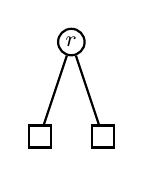
\begin{tikzpicture}
[-,thick,%
  every node/.style={shape=circle,inner sep=1.5pt,draw,thick},%
  scale=0.8]
\footnotesize
\node {$r$}
  [sibling distance=1cm]
  child {node[rectangle,inner sep=4pt,draw,thick] {}}
  child {node[rectangle,inner sep=4pt,draw,thick] {}};
\end{tikzpicture}
}
%%
%%
\qquad
\subfigure[]{

\begin{tikzpicture}
[-,thick,%
  every node/.style={shape=rectangle,inner sep=4pt,draw,thick},%
  scale=0.8]
\footnotesize
\node {};
\end{tikzpicture}
}
\end{figure}

\end{document}
